\documentclass[12pt]{book}
\usepackage[a4paper,bindingoffset=0.2in,%
            left=0.75in,right=0.75in,top=1in,bottom=1in,%
            footskip=.25in]{geometry}
\usepackage{fancyhdr}
\setlength{\headheight}{15.2pt}
\usepackage[utf8]{inputenc}
\pagestyle{fancy}

\renewcommand{\chaptermark}[1]{\markboth{\thechapter.\ #1}{}}
\renewcommand{\sectionmark}[1]{\markright{\thesection\ #1}}
\fancyhead[LE,RO]{\textbf{\thepage}}
\fancyhead[LO]{\textbf{\rightmark}}
\fancyhead[RE]{\textbf{\leftmark}}
\fancyfoot{}
\fancypagestyle{plain}
{
    \fancyhf{}
}


\usepackage{amsmath}
\usepackage{amssymb}
\usepackage{mathtools}
\usepackage{xcolor}
\usepackage{enumitem}
\usepackage{listings}
\usepackage[ruled,noline]{algorithm2e}
\usepackage{graphicx}
\usepackage{common}
\usepackage{english-theorems}
\setcounter{tocdepth}{1}

\definecolor{listinggray}{gray}{0.9}
\definecolor{lbcolor}{rgb}{0.9,0.9,0.9}
\definecolor{Darkgreen}{rgb}{0,0.4,0}
\lstdefinestyle{customc}{
    backgroundcolor=\color{lbcolor},
    tabsize=4,
  language=C++,
  captionpos=b,
  tabsize=3,
  frame=lines,
  numbers=left,
  numberstyle=\tiny,
  numbersep=5pt,
  breaklines=true,
  showstringspaces=false,
  basicstyle=\footnotesize,
%  identifierstyle=\color{magenta},
  keywordstyle=\color[rgb]{0,0,1},
  commentstyle=\color{Darkgreen},
  stringstyle=\color{red}
}

\lstnewenvironment{codeC}{
 \lstset{escapechar=@,style=customc}\bgroup
}{
    \egroup
}

\begin{document}
\tableofcontents
\clearpage
\ifodd\value{page}\else
\thispagestyle{empty}
\fi
\chapter{Kernel Abstraction}

\section{The process concept}
\chapter{Programming Interface}
what functionalities does the operating system provide applications 
\begin{description}
    \item[Process management:] start another process? wait for it to complete? signals?
    \item[Input/Output:] How to communicate with devices? how to communicate with another process.
    \item[Thread management:] multithreading? synchronization of data?
    \item[Memory management:] how to allocate more/less memory? can it share memory with other processes?
    \item[File system ans storage]
    \item[Networking and distribute systems:] how to commuincate with other computers?
    \item[Graphic and window management:] how to control its window? how to use graphical devices and accelerators?
    \item[Authentication and security:] what permission does it have?        
\end{description}

where to implement functionalities
\begin{itemize}
    \item user-level program. e.g. user login
    \item user-level library; linked to program. e.g. OS libs 
    \item kernel; accessed through system call. e.g. low level file I/O
    \item standalone server process; access through system calls and invoked by kernel. e.g. windows manager.
\end{itemize}

tradeoffs to consider 
\begin{description}
    \item[Flexibility:] easier if it is outside kernel.
    \item[Safety:] protection must be implemented in kernel.
    \item[Reliability:] keeping kernel minimal.
    \item[Performance:] transferring control between kernel and user is expensive.    
\end{description}
\section{Process management}
shell is a job control system. In Windows, processes are created by a system call.
\begin{codeC}
    CreateProcess()
\end{codeC}

In UNIX,
\begin{codeC}
    fork(); // copies parent process into child
    exec(); // copies a new program and start running it.
\end{codeC}
\begin{enumerate}
    \item UNIX fork 
    \begin{itemize}
        \item create and initialize PCB in kernel.
        \item create a new address space.
        \item initialize the address space with the copy of the entire contents of the address space of the parent.
        \item inherit the execution context. e.g. file descriptors
        \item inform scheduler that a new process is ready to run.
        \item it returns twice; for parent it returns the pid of the child and for child it returns 0.
    \end{itemize}
    \item UNIX exec 
    \begin{itemize}
        \item load program into current address space.
        \item copy args into memory in address space.
        \item initialize hardware context to start execution at ``start''.
    \end{itemize}
    \item UNIX wait
    \begin{itemize}
        \item waits for a particular child.
        \item running in background by appending an `\&'.
    \end{itemize}
\end{enumerate}
\subsection{Input/Output}
everything is a file. 
\begin{description}
    \item[Uniformity:] all I/O, file descriptors, IPC, etc use the same set of system calls.
    \item[Open before use:] check access permissions and do some bookkeeping.
    \item[Byte oriented:]  everything is accessed with byte arrays.
    \item[Kernel buffered read/writes] 
    \item[Explicit close] otherwise garbage collector.     
\end{description}
For IPC we need two or more system calls.
\subsubsection*{Pipe}
the pipe closes when either ends close the pipe or exit.
\begin{itemize}
    \item replace file descriptors with dup and dup2
    \item wait for multiple reads with select, allows the server to wait for input from any of a set of file descriptors; it returns the file descriptors that has data but does not read the data.
\end{itemize}

\subsection{Operating system structure}
\subsubsection*{Monolithic OS}
most OS functionalities run in kernel. to improve portability adds hardware abstraction layer and dynamically loaded device drivers. HAL is a portable interface to machine specific operations. Dynamically installed device drivers decouples OS kernel from specific devices (90\% bugs are here rather than OS itself).
\subsubsection*{Microkernel}
minimal kernel
\chapter{Slides}
\section{Lecture 1}
The key building blocks of OS
\begin{itemize}
    \item Process 
    \item Threads, Concurrency, Scheduling, Coordination
    \item Address space
    \item Protection, Isolation, Sharing , Security
    \item Communication, Protocols
    \item Persistent storage, Transaction, Consistency, Resilience
    \item Interfaces all devices
\end{itemize}

\begin{figure}
    \centering
    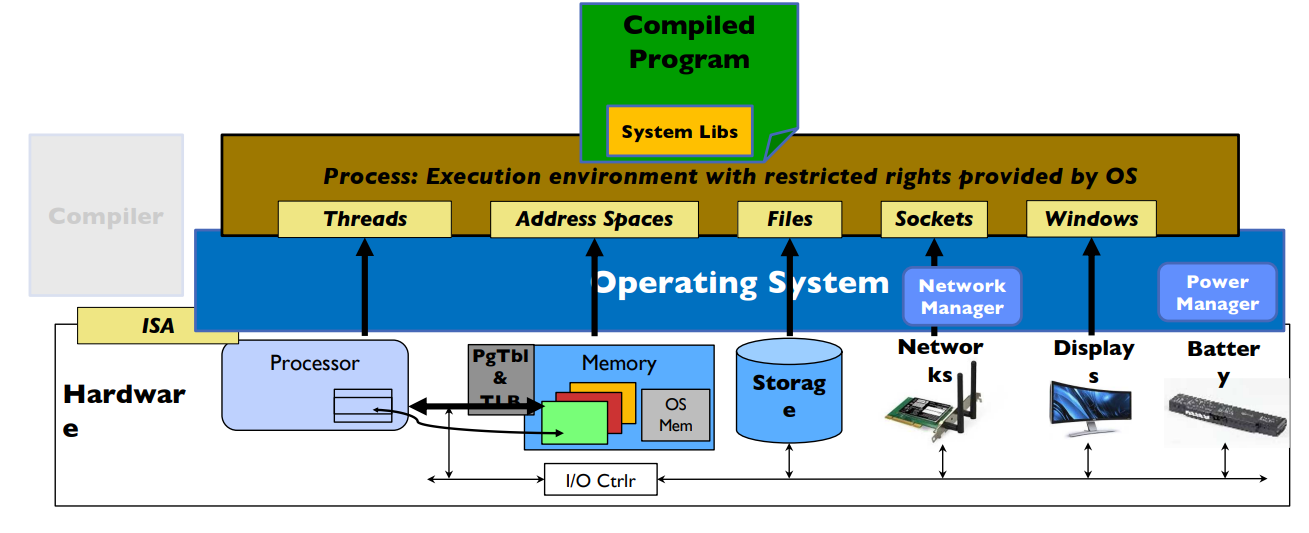
\includegraphics[width = 0.9\textwidth]{Chapters/graphics/OSAbstraction.png}
\end{figure}

\section{Lecture 2}
\subsection{Thread}
A single unit execution context 
\begin{itemize}
    \item It has program counter (PC), registers, execution flags, stack, and memory state
    \item A thread executes on a processor when it is \underline{resident} in the processor's register.
    \item A thread is suspended when its state is not load into processor.
    \item When a thread is not running it's saved in the memory called \underline{thread control unit (TCB)}. 
    \item TCB is saved in kernel.
\end{itemize}

\subsection{Address space}
The set of accessible address and the state associated with them.

\subsection{}
An operating system must 
\begin{itemize}
    \item protect itself from user programs.
    \item be reliable.
    \item be secure.
    \item ensure privacy.
    \item ensure fairness.
    \item protect programs from one another.
    \item prevent threads owned by one program to impact other
\end{itemize}
\subsection{Simple protection: Base and Bound (B\&B)}
sets lower and upperbound for a program to access.

\subsection{Process}
execution enviroment with restricted access. 
\begin{itemize}
    \item (Protected) address space with one or more threads
    \item owns memory
    \item has file descriptors, file system context
    \item encapsulate one or more therad sharing process resources.
\end{itemize}

\subsection{Dual mode}
\begin{enumerate}
    \item Kernel mode (superivor)
    \item User mode
\end{enumerate}

\section{Lecture 3}
\subsection{Motivation for threads}
Operating system needs to handle multiple things at once.
\begin{description}
    \item[Multiprocessing:] multiple CPU.
    \item[Multiprogramming:] multiple jobs/processes.
    \item[Multithreading:] multiple threads.   
\end{description}
Threads are mainly in three states 
\begin{enumerate}
    \item Running: running.
    \item Ready: eligible to run.
    \item Blocked: ineligible to run.
\end{enumerate}

\subsection{pthreads API}
\begin{description}
    \item[pthread\_create]
    \item[pthread\_exit] 
    \item[pthread\_join] suspends the execution calling thread until the target thread terminates.  
\end{description}

to avoid race conditions
\begin{itemize}
    \item Mutual exclusion: ensuring only one thread does a particular thing at a time.
    \item Critical sections: code exactly one thread can execute at a time.
\end{itemize}

\subsubsection*{Locks}
\begin{description}
    \item[acquire:] wait until lock is free.
    \item[release:] mark lock as free.  
\end{description}
both these operations are atomic. and done with pthread\_mutex\_init,lock,unlock.

\subsubsection*{Process}
Bootstrapping: every process is created from another process. first process is started by the kernel and is often called the init process.

\begin{description}
    \item[exit:] exits a process.
    \item[fork:] creates a brand new process and copies the whole process image.
    \item[exec:] changes the program being run.
    \item[wait:] wait for a process to finish.
    \item[kill:] send a signal to another process.
    \item[sigaction:] set handlers for signals.      
\end{description}

\section{Lecture 4}
\subsection{Semaphores}
Semaphores are non-negative integers.
\begin{description}
    \item[P()/down():]  atomic operation that waits for the semaphore to become positive, then decrement it by one.
    \item[V()/up():] atomic operation that increments semaphore by one, waking up a waiting process if any. 
\end{description}
\subsection{File system abstraction}
\begin{description}
    \item[File:] collection of data in a file system. 
    \item[Directory:] Hierarchical naming, links, volumes. 
\end{description}
every process has a current working directory.

\begin{description}
    \item[Absolute path:] /home/.
    \item[Relative path:] ../ for parent, ./ for current, ~/ for absolute path and a function of shell.  
\end{description}

\subsection{High level file API- Streams}
files are treated as unformated sequence of bytes.
FILE* fopen(,)

Key UNIX I/O design concepts 
\begin{itemize}
    \item Uniformity: everything is a file.
    \item Open before use
    \item Byte oriented
    \item Kernell buffered reads and writes
    \item Explicit close
\end{itemize}
open, creat, close,
int open() returns a file descriptor. open file descriptos are in kernel.
\subsubsection{Operation specific to terminals, devices, networking}
\begin{enumerate}
    \item ioctl()
    \item dup(), dup2()
    \item pipe()
    \item file locking
    \item memory mapping files
\end{enumerate}

\section{Lecture 5}
\subsection{Interprocess Communication (IPC)}
Communication between two or more processes. One way; data written by process A is held in memory until B reads it.
\subsubsection{UNIX pipe}
A writes to pipe, B reads from pipe.
\begin{itemize}
    \item If producer tries to write when buffer is full; it blocks.
    \item If consumer tries to read when buffer is empty; it blocks.
\end{itemize}
int pip(int fileds[2]);
\begin{itemize}
    \item allocates two new file descriptors in the process.
    \item writes to fileds[1] and reads from fileds[0].
    \item Implemented as fixed size queue inside kernel memory.
    \item After read file descriptor closes, writes generates SIGPIPE. If process ignores, then the write fails with an EPIPE error.
    \item After write file descriptor closes, pipe is effectively closed and reads return EOF.
\end{itemize}

A protocol is an agreement on how to communicate. which covers syntax and semantics.
Client server protocols: Cross network IPC.
Client initiates contact and server responses.
key idea: communication looks like file I/O.
\end{document}